\documentclass[reqno]{amsart}

\usepackage{amsfonts,latexsym,amsthm,amssymb,amsmath,amscd,euscript,bm}
\usepackage[sc]{mathpazo}
\usepackage[margin = 2cm]{geometry}
\usepackage{enumitem}
\usepackage{hyperref}
% sets numbering of enumerate to a, b, c, ...
\renewcommand{\theenumi}{\alph{enumi}}

% Theorems, propositions, etc.
\newtheorem{theorem}{Theorem}
\newtheorem{proposition}[theorem]{Proposition}
\newtheorem{lemma}[theorem]{Lemma}
\newtheorem{corollary}[theorem]{Corollary}

\theoremstyle{definition}
\newtheorem{definition}[theorem]{Definition}
\newtheorem*{claim}{Claim}

\theoremstyle{remark}
\newtheorem*{remark}{Remark}
\newtheorem*{notation}{Notation}

\usepackage{tikz-cd}

\usepackage{thmtools}
\usepackage[framemethod=TikZ]{mdframed}
	\mdfdefinestyle{mdrecbox}
		{%
			linewidth=0.5pt,
			skipabove=12pt,
			frametitleaboveskip=5pt,
			frametitlebelowskip=0pt,
			skipbelow=2pt,
			frametitlefont=\bfseries,
			innertopmargin=4pt,
			innerbottommargin=8pt,
			nobreak=true,
		}
	\declaretheoremstyle
		[
			headfont=\bfseries,
			mdframed={style=mdrecbox},
			headpunct={\\[3pt]},
			postheadspace={0pt},
		]
		{thmrecbox}
\newcounter{problem}[section]	\declaretheorem[style=thmrecbox,name=Problem, numberlike=problem]{statement}


% Solution environment
\newenvironment{solution}
	{
		\begin{proof}[Solution]}{\end{proof}
	}


% Math blackboard font
\newcommand{\nc}{\newcommand}
\nc{\on}[1]{\operatorname{#1}}

\nc{\R}{\mathbb R}
\nc{\C}{\mathbb C}
\nc{\Q}{\mathbb Q}
\nc{\Z}{\mathbb Z}
\nc{\N}{\mathbb N}
\nc{\HH}{\mathbb H}
\nc{\DD}{\mathbb D}
\nc{\TT}{\mathbb T}
\nc{\EE}{\mathbb E}
\nc{\PP}{\mathbb P}

\nc{\cT}{\mathcal T}
\nc{\cA}{\mathcal A}
\nc{\cM}{\mathcal M}
\nc{\cR}{\mathcal R}
\nc{\cB}{\mathcal B}
\nc{\cG}{\mathcal G}
\nc{\cD}{\mathcal D}
\nc{\cS}{\mathcal S}
\nc{\cF}{\mathcal F}
\nc{\cL}{\mathcal L}
\nc{\cE}{\mathcal E}

\nc{\diam}{\operatorname{diam}}
\nc{\del}{\partial}
\nc{\osc}{\operatorname{osc}}
\nc{\inter}{\mathrm{o}}
\nc{\close}[1]{\overline{#1}}
\nc{\supp}{\operatorname{supp}}
\nc{\BV}{\operatorname{BV}}
\nc{\Per}{\operatorname{Per}}
\nc{\loc}{\text{loc}}
\nc{\Lip}{\operatorname{Lip}}
\nc{\ACL}{\operatorname{ACL}}

% Why the f*** would you ever use \epsilon
\renewcommand{\epsilon}{\varepsilon}
\renewcommand{\emph}{\textsc}
\renewcommand{\Re}{\operatorname{Re}}
\renewcommand{\Im}{\operatorname{Im}}
%inverse Fourier transform widecheck
\DeclareFontFamily{U}{mathx}{\hyphenchar\font45}
\DeclareFontShape{U}{mathx}{m}{n}{
      <5> <6> <7> <8> <9> <10>
      <10.95> <12> <14.4> <17.28> <20.74> <24.88>
      mathx10
      }{}
\DeclareSymbolFont{mathx}{U}{mathx}{m}{n}
\DeclareFontSubstitution{U}{mathx}{m}{n}
\DeclareMathAccent{\widecheck}{0}{mathx}{"71}

\let\vec\mathbf

% Title: change problem set number as needed
\title
{
	\emph{Heat equation}
} 

\author{Jason Zhao}
\date{\today}

\begin{document}
\maketitle

\begin{abstract}
	The prototypical example of a parabolic partial differential equation is the \textit{heat equation},
		\[ \partial_t u - \Delta u = f. \]
	This equation models	 heat flow. 
\end{abstract}

\tableofcontents

\section{Fundamental solution}

The \emph{fundamental solution} of the heat operator is a distribution $K \in C^\infty_c (\R^{1 + d})^*$ such that 
	\[  (\partial_t - \Delta) K = \delta_0. \]
In terms of thermodynamics, we view the fundamental solution as the heat flow arising from the unit heat source concentrated at the origin. We can construct solutions to the heat equation on $\R^{1 + d}$ by convolving the fundamental solution with the source term; for any compactly supported distribution $f\in C^\infty (\R^{1 + d})^*$, we have
	\[ f = \delta_0 * f = (\partial_t - \Delta)K * f = \Delta (K * f). \]
The fundamental solution takes the form 
	\[ K(t, x) := \frac{1}{(4\pi t)^{d/2}} e^{-x^2/4t} \mathbb 1_{t > 0} (t). \]

\subsection{Derivation}

Applying the space-time Fourier transform, the fundamental solution satisfies 
	\[ (2\pi i \tau + 4\pi^2 |\xi|^2) \cF_{t, x} K = 1. \]
Formally rearranging, we can write
	\[ \cF_{t, x} K = \frac{1}{2\pi i \tau + 4\pi^2 |\xi|^2}.  \]
Assuming $d \geq 2$, the singularity at $(\tau, \xi) = (0, 0)$ is integrable, so the right-hand side is well-defined as a tempered distribution and the fundamental solution is given as a inverse space-time Fourier transform. Note that we can write $\cF_{t, x} = \cF_t \cF_x$; it will be convenient to first invert in the time variable. Appealing to continuity of $\cF_t : \cS^*_t (\R) \to \cS^*_t (\R)$ and convergence of the Fourier integral on $L^1_t (\R)$, we can write
	\begin{align*}
		\cF^{-1}_\tau \left(\frac{1}{2\pi i \tau + 4\pi^2 |\xi|^2} \right)(t) 
			&=
		\lim_{R \to \infty} \cF^{-1}_\tau \left( \frac{1}{2\pi i \tau + 4\pi^2 |\xi|^2} \mathbb 1_{[-R, R]} (\tau) \right) (t) \\
			&=			
			\lim_{R \to \infty} \int_{[-R, R]} \frac{e^{2\pi i t \tau}}{2\pi i \tau + 4\pi^2 |\xi|^2} d \tau.
		\end{align*} 	
	To compute the Fourier integral explicitly, we argue by the residue theorem, viewing the integrand as a meromorphic function in $\tau$. We know from the Jordan lemma that the integral over the upper (lower) semi-circle contours of radius $R$ vanish for $t > 0$ ($t < 0$) as $R \to \infty$, so the limit converges to the residue at $\tau = 2\pi i |\xi|^2$ for $t > 0$ and vanishes for $t < 0$,
		\[ \lim_{R \to \infty} \int_{[-R, R]} \frac{e^{2\pi i t \tau}}{2\pi i \tau + 4\pi^2 |\xi|^2} d \tau =   e^{- 4\pi^2 t |\xi|^2} \mathbb 1_{t > 0} (t) \]
	This is a Gaussian in $\xi$, so taking the inverse Fourier transform in the spatial frequency $\xi$ produces the following fundamental solution, 
	\[ K(t, x) = \cF^{-1}_{\tau, \xi}\left( \frac{1}{2\pi i\tau + 4\pi^2 |\xi|^2} \right) = \cF_{\xi}^{-1}\left(   e^{-4\pi^2 t |\xi|^2} \mathbb 1_{t > 0} (t) \right)   = \frac{1}{(4\pi t)^{d/2}} e^{-|x|^2/4t} \mathbb 1_{t > 0} (t). \]
We remark that $K$ is smooth away from the origin, which implies the heat operator is \textit{hypoelliptic}, that is, following the proof of Weyl's lemma for Laplace's equation, we have the following result, 
	
\begin{theorem}[$C^\infty$-hypoelliptic regularity]
	Let $\Omega \subseteq \R^{1 + d}$ and suppose $\phi \in C^\infty_c (\Omega)^*$ is a distributional solution to the heat equation 
		\[ (\partial_t - \Delta)\phi = f \]
	for $f \in C^\infty (\Omega)$. Then $\phi$ is smooth. 	
\end{theorem}

\subsection{Propagator}

Let $\phi \in C^1_t \cS_x^* (\R \times \R^d)$ be a distributional solution to the free heat equation subject to initial data $\phi_0 \in \cS_x^* (\R^d)$. Converting from spatial physical space to spatial frequency space via the spatial Fourier transform, the PDE in space-time takes the form of an ODE in time, 
	\begin{align*}
		\partial_t \widehat \phi + 4\pi |\xi|^2 \widehat \phi
			&= 0, \\
		\widehat \phi_{|t = 0}
			&= \widehat{\phi_0}.
	\end{align*}
This admits the unique solution 
	\[ \widehat \phi (t, \xi) = e^{-4\pi |\xi|^2 t} \widehat{\phi_0} (\xi). \]	
Converting back to spatial physical space, we can write the solution to the free heat equation as 
	\[ \phi(t, x) = e^{t \Delta} \phi_0 (x) \]	
where $e^{t \Delta}$ is a Fourier multiplier known as the \emph{heat propagator}. By variation of parameters, we can construct a solution to the inhomogeneous heat equation as a superposition of free solutions with initial data from the forcing term $f$;

\begin{theorem}[Duhamel's formula]
	Suppose $\phi_0 \in \cS^*_x (\R^d)$ and $f \in C^0_t \cS_x^* ([0, T] \times \R^d)$. Then $\phi \in C^1_t \cS_x^* ([0, T] \times \R^d)$ defined by the formula
		\[ \phi(t) := e^{t \Delta} \phi_0 +  \int_0^t e^{(t - s) \Delta} f(s) \, ds \]
	solves the heat equation $(\partial_t - \Delta) \phi = f$ with initial data $\phi_{|t = 0} = \phi_0$. 	
\end{theorem}

\begin{proof}
	We make the \textit{ansatz} that the solution takes the form $\phi = e^{t \Delta} \psi$, then $\psi$ satisfies the equation 
		\[ e^{t \Delta} \partial_t \psi = (\partial_t - \Delta) e^{t \Delta} \psi = f \]
	with initial data $\psi_{|t = 0} = \phi_0$. Rearranging and applying the fundamental theorem of calculus, we obtain 
		\[ \psi(t) = \phi_0 + \int_0^t e^{-s \Delta} f(s) \, ds.  \]
	This proves the result. 		
\end{proof}	

\begin{remark}
	We can view the fundamental solution as the heat propagation of the Dirac delta initial data, 
		\[ K(t) = e^{t \Delta} \delta_{x = 0} = \int_{\R^d} e^{-4\pi^2 t|\xi|^2} e^{2\pi i x \cdot \xi} \, d\xi. \]
\end{remark}

\begin{corollary}[Energy estimates]
	For $s \in \R$, let $\phi_0 \in H^s_x (\R^d)$ and $f \in L^1_t H^s_x ([0, T] \times \R^d)$. Then the solution to the heat equation $(\partial_t - \Delta) \phi = f$ with initial data $\phi_{|t = 0} = \phi_0$ satisfies
		\begin{align*}
			|| \phi||_{C^0_t H^s_x} + ||\nabla_x \phi||_{L^2_t H^s_x} \lesssim ||\phi_0||_{H^s_x} + ||f||_{L^1_{t} H^s},\\
		\end{align*}	\label{cor:energy}
\end{corollary}

\begin{proof}
	By the triangle inequality, Minkowski's integral inequality, Plancharel's theorem, and $L^2$-boundedness of Fourier multipliers, 
		\begin{align*}
			 || \phi||_{H^s_x} (t) 
			 	&\lesssim ||e^{t \Delta} \phi_0 ||_{H^s_x} + \int_0^t ||e^{(t - s) \Delta} f||_{H^s_x} (t') dt' \lesssim ||\phi_0||_{H^s_x} + || f||_{L^1_t H^s_x}, 	  
		\end{align*}	 
	and
		\[ ||\nabla_x \phi ||_{L^2_t H^s_x} \]	
\end{proof}

\begin{corollary}[First law of thermodynamics]
	Let $\phi \in C^1_t L^1_x ([0, T] \times \R^d)$ be a solution to the free heat equation. Then the mass functional
		\[ M[\phi](t) := \int_{\R^d} \phi \, dx \]
	is constant in time. 	
\end{corollary}

\begin{proof}
	The solution satisfies the following identity in spatial frequency space, 
		\[ M[\phi](0) = \widehat \phi (t, 0) = \widehat{\phi_0} (0) = \int_{\R^d} \phi_0 \, dx, \]
	as desired. 	
\end{proof}

\begin{corollary}[Second law of thermodynamics]
	Let $\phi \in C^1_t L^2_x ([0, T] \times \R^d)$ be a solution to the free heat equation. Then the energy functional
		\[ E[\phi](t) := \frac12 ||\phi||_{L^2_x}^2 (t) \]
	is non-increasing. 
\end{corollary}

\begin{proof}
	The multiplier $t \mapsto e^{-4\pi^2 t|\xi|^2}$ is decreasing, so the result follows from Plancharel. 
\end{proof}

\section{Maximum principle}

The second law of thermodynamics states that heat moves from hotter regions to cooler regions unless additional energy is supplied. With this physical intuition, we expect solutions $\phi : [0, T] \times \Omega \to \R$ to the free heat equation $(\partial_t - \Delta) \phi = 0$ to obey the \textit{strong maximum principle}, non-constant solutions cannot achieve a maximum on the \emph{parabolic interior}
	\[ \Omega_T := \Omega \times (0, T]. \]
The \textit{weak maximum principle} follows as a direct corollary, stating if $\phi$ extends continuously to the boundary, then it achieves its maximum on the \emph{parabolic boundary}
	\[ \Gamma_T := \overline{\Omega_T} \setminus \Omega_T.  \]
More generally, we say that a function $\phi: [0, T] \times \Omega \to \R$ is a \emph{sub-solution} to the heat equation if
	\[ (\partial_t - \Delta) \phi \leq 0. \]
Sub-solutions correspond to heat distributions with negative source term, and thus also satisfy the strong and weak maximum principles. 	
	
\begin{figure}[h]
	\begin{center}
		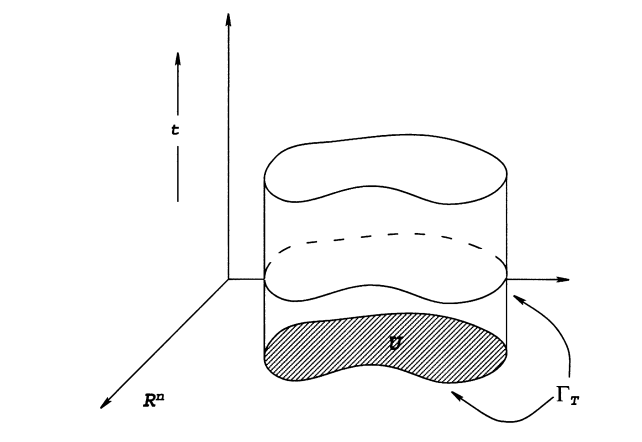
\includegraphics[scale =0.6]{parabolic}
		\caption{The parabolic boundary $\Gamma_T \subseteq [0, T] \times \overline\Omega$ consists of the bottom and vertical sides of the parabolic interior.}
	\end{center}
\end{figure}

\subsection{Mean value property}

Our proof of the maximum principle will rely on a mean value characterisation of sub-solutions. Define the \emph{heat ball} as the super-level sets of the fundamental solution 
	\[ E_r (t, x) := \{ (s, y) \in (-\infty, t] \times \R^d : K(x - y, t - s) \geq \frac{1}{r^d} \}. \]
Observe that 
	\[ \frac{1}{4r^d}\int_{E_r (t, x)} \frac{|x - y|^2}{(t - s)^2} \, dy ds = 1. \]	

\begin{theorem}[Sub-mean value property]
	Let $\phi \in C^1_t C^2_x (\Omega_T)$ be a sub-solution to the heat equation. Then 
		\[ \phi(t, x) \leq \frac{1}{4r^d} \int_{E_r (t, x)} \phi(y, s) \frac{|x - y|^2}{(t - s)^2} dy ds \]
	for each $E_{r} (t, x) \subseteq \Omega_T$. 	
\end{theorem}

\begin{proof}
	Translating in space and time, we can assume without loss of generality $(t, x) = (0, 0)$. We argue by a monotonicity formula, defining
		\[ \Phi(r) := \frac{1}{r^d} \int_{E_r (0, 0)} \phi(y, s) \frac{|x - y|^2}{(t - s)^2} dy ds = \int_{E_1 (0, 0)} \phi(r^2 s, ry) \frac{|y|^2}{s^2} dy ds . \]
	To conclude the sub-mean value property, it would suffice to show $\Phi$ is non-decreasing in $r$ since $\Phi(r) \to \phi(t, x)$ as $r \to 0$ by continuity of $\phi$. Differentiating and rescaling,
		\begin{align*}
			\Phi'(r)
				&= \int_{E_1 (0, 0)} \left(y \cdot \nabla_y u (r^2 s, r y)   \frac{|y|^2}{s^2} + 2r \partial_s u (r^2 s, ry)  \frac{|y|^2}{s}\right)  \, dy ds \\
				&= \frac{1}{r^{d + 1}} \int_{E_r (0, 0)} \left(y \cdot \nabla_y u (s, y) \frac{|y|^2}{s^2}  + 2 \partial_s u (s, y) \frac{|y|^2}{s}  \right) \, dy ds =: \text{I} + \text{II}.
		\end{align*}
	Define $\psi : E_r (0, 0) \to \R$ by 
		\[ e^{\psi (y, s)} := \frac{1}{r^d} \frac{1}{(-4\pi s)^{d/2}} e^{|y|^2/4s}\]
	and observe that $\psi \equiv 0$ on $\partial E_r (0, 0)$ since $K(y, -s) \equiv r^{-d}$ on $\partial E_r (0, 0)$. 
\end{proof}

\begin{corollary}[Mean value property]
	Let $\phi \in C^1_t C^2_x (\Omega_T)$ be a solution to the free heat equation $(\partial_t - \Delta) \phi = 0$. Then 
		\[ \phi(t, x) = \frac{1}{4r^d} \int_{E_r (t, x)} \phi(y, s) \frac{|x - y|^2}{(t - s)^2} dy ds \]
	for each $E_{r} (t, x) \subseteq \Omega_T$. 	
\end{corollary}

\begin{proof}
	If $\phi$ is a solution to the free heat equation, then the proof of the sub-mean value property continues to hold replacing $\phi$ with $-\phi$, which furnishes equalities in place of the inequalities.
\end{proof}

\subsection{Maximum principles}

\begin{theorem}[Strong maximum principle]
	Let $\Omega \subseteq \R^d$ be a bounded domain, and suppose $u \in C^1_t C^2_x ([0, T] \times \Omega)$ solves the heat equation. If $u$ achieves its maximum, i.e. there exists $(t_0, x_0) \in \Omega_T$ such that 
		\[ u(t_0, x_0) = \sup u ([0, T] \times \Omega) \]
	then $u$ is constant. 	
\end{theorem}

\begin{proof}
	
\end{proof}

\begin{corollary}[Weak maximum principle]
	Let $\Omega \subseteq \R^d$ be a bounded domain, and suppose $u \in C^1_t C^2_x (\Omega \times [0, T])$ solves the heat equation. If $u$ extends continuously to the boundary, then it achieves its maximum on the parabolic boundary, i.e.
		\[ \sup u (\Gamma_T) = \sup u ([0, T] \times \Omega) \]
\end{corollary}

\begin{corollary}[Comparison principle]
	Let $\Omega \subseteq \R^d$ be a bounded domain, and suppose $u, v : [0,T] \times \Omega \to \R$ are sub-solutions and super-solutions respectively extending continuously to the boundary. If $u \leq v$ on the parabolic boundary $\Gamma_T$, the $u \leq v$ on the entire domain $[0, T] \times \Omega$. 
\end{corollary}

\begin{proof}
	The difference $u - v$ is a sub-solution on $[0, T] \times \Omega$ extending continuously to the boundary, so it obeys the weak maximum principle, i.e. the maximum is on the parabolic boundary. Since $u - v \leq 0$ on the parabolic boundary, we have $u - v \leq 0$ on $[0, T] \times \Omega$. 
\end{proof}

\begin{theorem}[Maximum principle on $\R^d$]
	Suppose $\phi \in C^1_t C^2_x ([0, T] \times \R^d)$ solves the free heat equation $(\partial_t - \Delta)\phi = 0$ with initial data $\phi_{|t = 0} = \phi_0$, and satisfies the growth estimate
		\[ |\phi(t, x)| \lesssim e^{a|x|^2}\]
	for some $a > 0$. Then 
		\[ \sup \phi ([0, T] \times \R^d)= \sup \phi_0 (\R^d). \]	
\end{theorem}

\begin{proof}
	We appeal to the Phragmen-Lindelof principle, introducing an auxiliary function which decays at $|x|\to \infty$, allowing us to apply the maximum principle on bounded domains. We prove the result assuming $4a (T + \delta) < 1$ for some $\delta > 0$. The general case would follow by decomposing 
		\[ [0, T] = [0, T/n] \cup [T/n, 2T/n] \cup \dots \cup [(n - 1)T/n, T] \]
	for $n \gg_a 1$ and applying the result on each sub-interval. 
	
	Assume then $4a (T + \delta) < 1$ for $\delta > 0$, i.e. $1/4(T + \delta) = a + \eta$ for some $\eta > 0$. For $\epsilon > 0$ and $y \in \R^d$ define 	
		\[ \phi_{\epsilon, y} (t, x) := \phi(t, x) - \frac{\epsilon}{(T + \delta - t)^{d/2}} e^{\frac{|x - y|^2}{4(T + \delta - t)}}. \]
	A direct computation shows that $\phi_{\epsilon, y}$ solves the heat equation. Fix $r > 0$ and set $\Omega := B_r (y)$. By the weak maximum principle on bounded domains, 
		\[ \max \phi_{\epsilon, y} (\Omega_T) = \max \phi_{\epsilon, y} (\Gamma_T). \]
	By construction, 
		\[ \phi_{\epsilon, y} (0, x) \leq \phi_0 (x)  \]	
	for all $x \in \R^d$, and 
		\[ \phi_{\epsilon, y} (t, x) \lesssim e^{a(|y| + r)^2} -\frac{\epsilon}{(T + \delta)^{d/2}} e^{\frac{r^2}{4(T + \delta)}} \leq e^{a(|y| + r)^2} - 4^{d/2}\epsilon (a + \eta)^{d/2} e^{(a + \eta) r^2} \]
	for $|x - y| = r$ and $t \in [0, T]$. Choosing $r \gg 1$, the right-hand side can be made arbitrarily negative, so collecting our results we can conclude
		\[ \phi_{\epsilon, y} (t, x) \leq \sup \phi_0 (\R^d) \]
	for $(t, x) \in \Gamma_T$. Applying the weak maximum principle, the inequality continues to hold for $(t, x) \in \Omega_T$. Taking $r \to \infty$ and $\epsilon \to 0$ completes the proof. 
\end{proof}

\begin{corollary}[Uniqueness on $\R^d$]
	Let $f \in C([0, T] \times \R^d)$ and $\phi_0 \in C (\R^d)$. Then there exists at most one solution $\phi \in C^1_t C^2_x ([0, T] \times \R^d)$ to the heat equation $(\partial_t - \Delta)\phi = f$ with initial data $\phi_{|t = 0} = \phi_0$ satisfying the growth estimate
		\[ |\phi(t, x)| \lesssim e^{a|x|^2}. \]
\end{corollary}

\begin{remark}
	There are in fact infinitely many solutions of 
		\begin{align*}
			(\partial_t - \Delta) \phi
				&= 0, \\
			\phi_{|t =0}
				&= 0.	
		\end{align*}
	It follows from uniqueness that each non-zero solution must grow rapidly as $|x| \to \infty$. The growth estimate excludes the possibility of an ``infinite'' heat source at $|x| = \infty$ which could be constructed to violate uniqueness via infinite speed of propagation. 
\end{remark}


\section{Energy methods}



Let $\Omega \subseteq \R^d$ be a $C^1$-domain, and suppose $f \in L^2_{t, x} ([0, T] \times \Omega)$ and $\phi_0 \in $

When working in general domains $\Omega \subseteq \R^d$. \ref{cor:energy}

We define the \emph{energy} of $u : \Omega \times (0, \infty) \to \R$ by 
	\[ E[u] := \frac12 || u||_{L^2_x (\Omega)}^2 (t) = \frac12 \int_\Omega |u(t, x)|^2 \, dx.  \]

\subsection{A priori estimate}

Suppose $u$ is a solution to the initial value problem with Dirichlet boundary conditions
	\begin{align*}
		\partial_t u - \Delta u
			&= f,\\
		u_{|t = 0}
			&= u_0, \\
		u_{|\partial \Omega}
			&= 0.	
	\end{align*}

\begin{theorem}[A priori estimate]
	For $s \in \R$, let $f \in L^1_t H^s_x ([0, T] \times \R^d)$ and suppose $\phi \in C^0_t H^s_x ([0, T] \times \R^d)$ is a solution to the heat equation $(\partial_t - \Delta) \phi = f$. Then
		\[ || \phi||_{C^0_t H^s_x} + ||\nabla_x \phi||_{L^2_t H^s_x} \lesssim ||\phi_0||_{H^s_x} + ||f||_{L^1_{t} H^s}. \]
\end{theorem}	
	
\begin{proof}
	Differentiating the energy, we obtain
		\[ \frac{d}{dt} E[u] (t) = \int_\Omega u \, \partial_t u \, dx = \int_\Omega u f \, dx + \int_\Omega u \Delta u \, dx = \int_\Omega u f \, dx - \int_\Omega |\nabla u|^2 \, dx, \]
	where we used the heat equation in the second equality and integration by parts in the third equality. Integrating in time, using the fundamental theorem of calculus on the left, we rearrange to obtain
		\begin{align*}
			 ||u||_{L^2_x}^2 (T_0) + || u ||_{L^2_t \dot H^1_x(0, T_0)}^2 
			 	&=  E[u] (T_0) + \int_0^{T_0} \int_\Omega |\nabla u|^2 \, dx dt \\
			 	&= \int_0^{T_0} \int_\Omega u f \, dx + E[u](0) = \int_0^{T_0} \int_\Omega u f \, dx + ||u_0||_{L^2_x}^2 
		\end{align*}	 	
	for any $0 \leq T_0 \leq T$. We control the first term on the right using Cauchy-Schwartz and the arithmetic-geometric mean inequality,  
		\begin{align*}
			\int_0^{T_0} \int_\Omega u f \, dx \leq ||f||_{L^2_{t, x} (0, T)} ||u||_{L^2_{t, x} (0, T)} \leq \frac{1}{4\epsilon} ||f||_{L^2_{t, x} (0, T)}^2 + \epsilon ||u||_{L^2_{t, x}(0, T)}^2 \leq \frac{1}{4\epsilon} ||f||_{L^2_{t, x} (0, T)}^2 + \epsilon T ||u||_{L^\infty_t L^2_x (0, T)}^2  
		\end{align*}	
	for any $\epsilon > 0$. Collecting our results and choosing $\epsilon = 1/4T$ furnishes the inequality. 
\end{proof}


\end{document}